\chapter{Исследовательская часть}

\section{Интерфейс приложения}

На рисунке~\ref{fig:interface} представлен интерфейс приложения.

\begin{figure}[h!]
	\centering{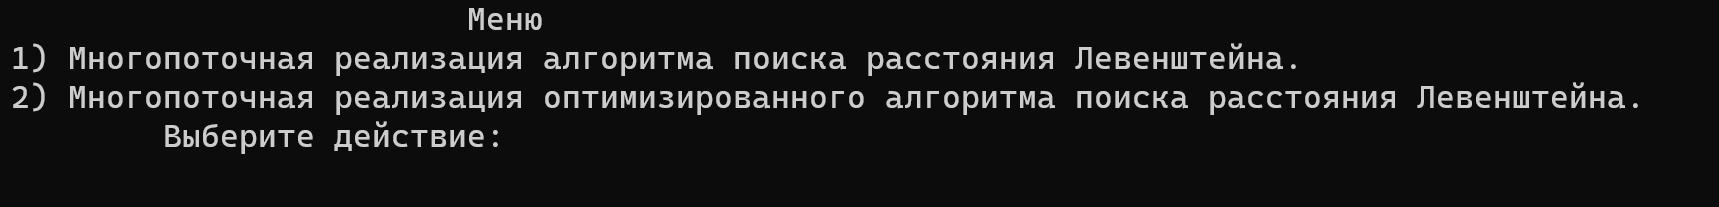
\includegraphics[scale=0.7]{photos/interface.png}}
	\caption{Интерфейс приложения}
	\label{fig:interface}
\end{figure}

\section{Технические характеристики}

Технические характеристики устройства:

\begin{itemize}
	\item операционная система --- Windows 11 Pro 64 -- разрядная система~\cite{windows};
	\item оперативная память --- 16 Гбайт;
	\item процессор --- 11th Gen Intel(R) Core(TM) i7-1165G7 с тактовой частотой 2.8 ГГц;
	\item количество ядер --- 4 физических и 8 логических ядер.
\end{itemize}

\section{Время выполнения реализаций алгоритмов}

На рисунке \ref{fig:graph1} приведено сравнение реализации алгоритма поиска расстояния Левенштейна и модифицированного алгоритма поиска расстояния Левенштейна. 
Время было найдено как среднее пяти измерений.

\begin{figure}[ht!]
	\begin{center}
		\captionsetup{singlelinecheck = false, justification=centerfirst}
		\begin{tikzpicture}
			\begin{axis}[
				xlabel={Количество ядер},
				ylabel={Время в секундах},
				width = 0.95\textwidth,
				height=0.5\textheight,
				xmin=0, xmax=16,
				ymode=log, 
				legend pos=north west,
				legend style={font=\footnotesize},
				xmajorgrids=true,
				grid style=dashed,
				]
				
				\addplot[
				blue,
				semithick,
				mark = *,
				mark size = 3pt,
				thick,
				] file {graph/multi_thread1.csv};
				
				\addplot[
				red,
				semithick,
				mark = x,
				] file {graph/multi_thread2.csv};
				
				\legend{
					Алгоритм поиска расстояния Левенштейна,
					Модифицированный алгоритм поиска расстояния Левенштейна
				}
			\end{axis}
			
		\end{tikzpicture}
		\centering
		\caption{Сравнение времени работы реализаций алгоритмов}
		\label{fig:graph1}
	\end{center}
\end{figure}
\clearpage

\section*{Вывод}

В ходе сравнения алгоритма поиска расстояния Левенштейна и модифицированного алгоритма поиска расстояния Левенштейна выявлено, что модифицированный алгоритм по времени быстрее работает. 
Этот успех объясняется несколькими ключевыми оптимизациями.

Прежде всего, модификация алгоритма включает в себя использование одномерного массива вместо матрицы для хранения расстояний между символами. 
Такой подход существенно экономит память и сокращает количество операций обращения к ней, что в итоге приводит к повышению общей производительности.

Дополнительно, внедрена дополнительная переменная, которая заменяет значения двух ячеек (arr[i-1][j-1] и arr[i][j-1]). 
Это уменьшает необходимость постоянного обращения к ячейкам матрицы в рамках каждой итерации цикла, что также способствует улучшению общей производительности алгоритма.

Кроме того, применен оптимизированный подход к расчету замены. 
Расчет стоимости замены осуществляется прямо внутри формулы для определения минимального значения, что сокращает время, требуемое для вычисления изменения, и, следовательно, повышает эффективность алгоритма в целом.